\section{Solución}

\subsection{Video}
Desarrollamos un video explicativo de la solución propuesta, pueden encontrarlo
en el siguiente \href{https://www.overleaf.com/learn/latex/Inserting_Images}{Link del video}.

\subsection{Descripción}
Dado todo el contexto del problema definimos la siguiente arquitectura.

\begin{figure}[h]
    \centering
    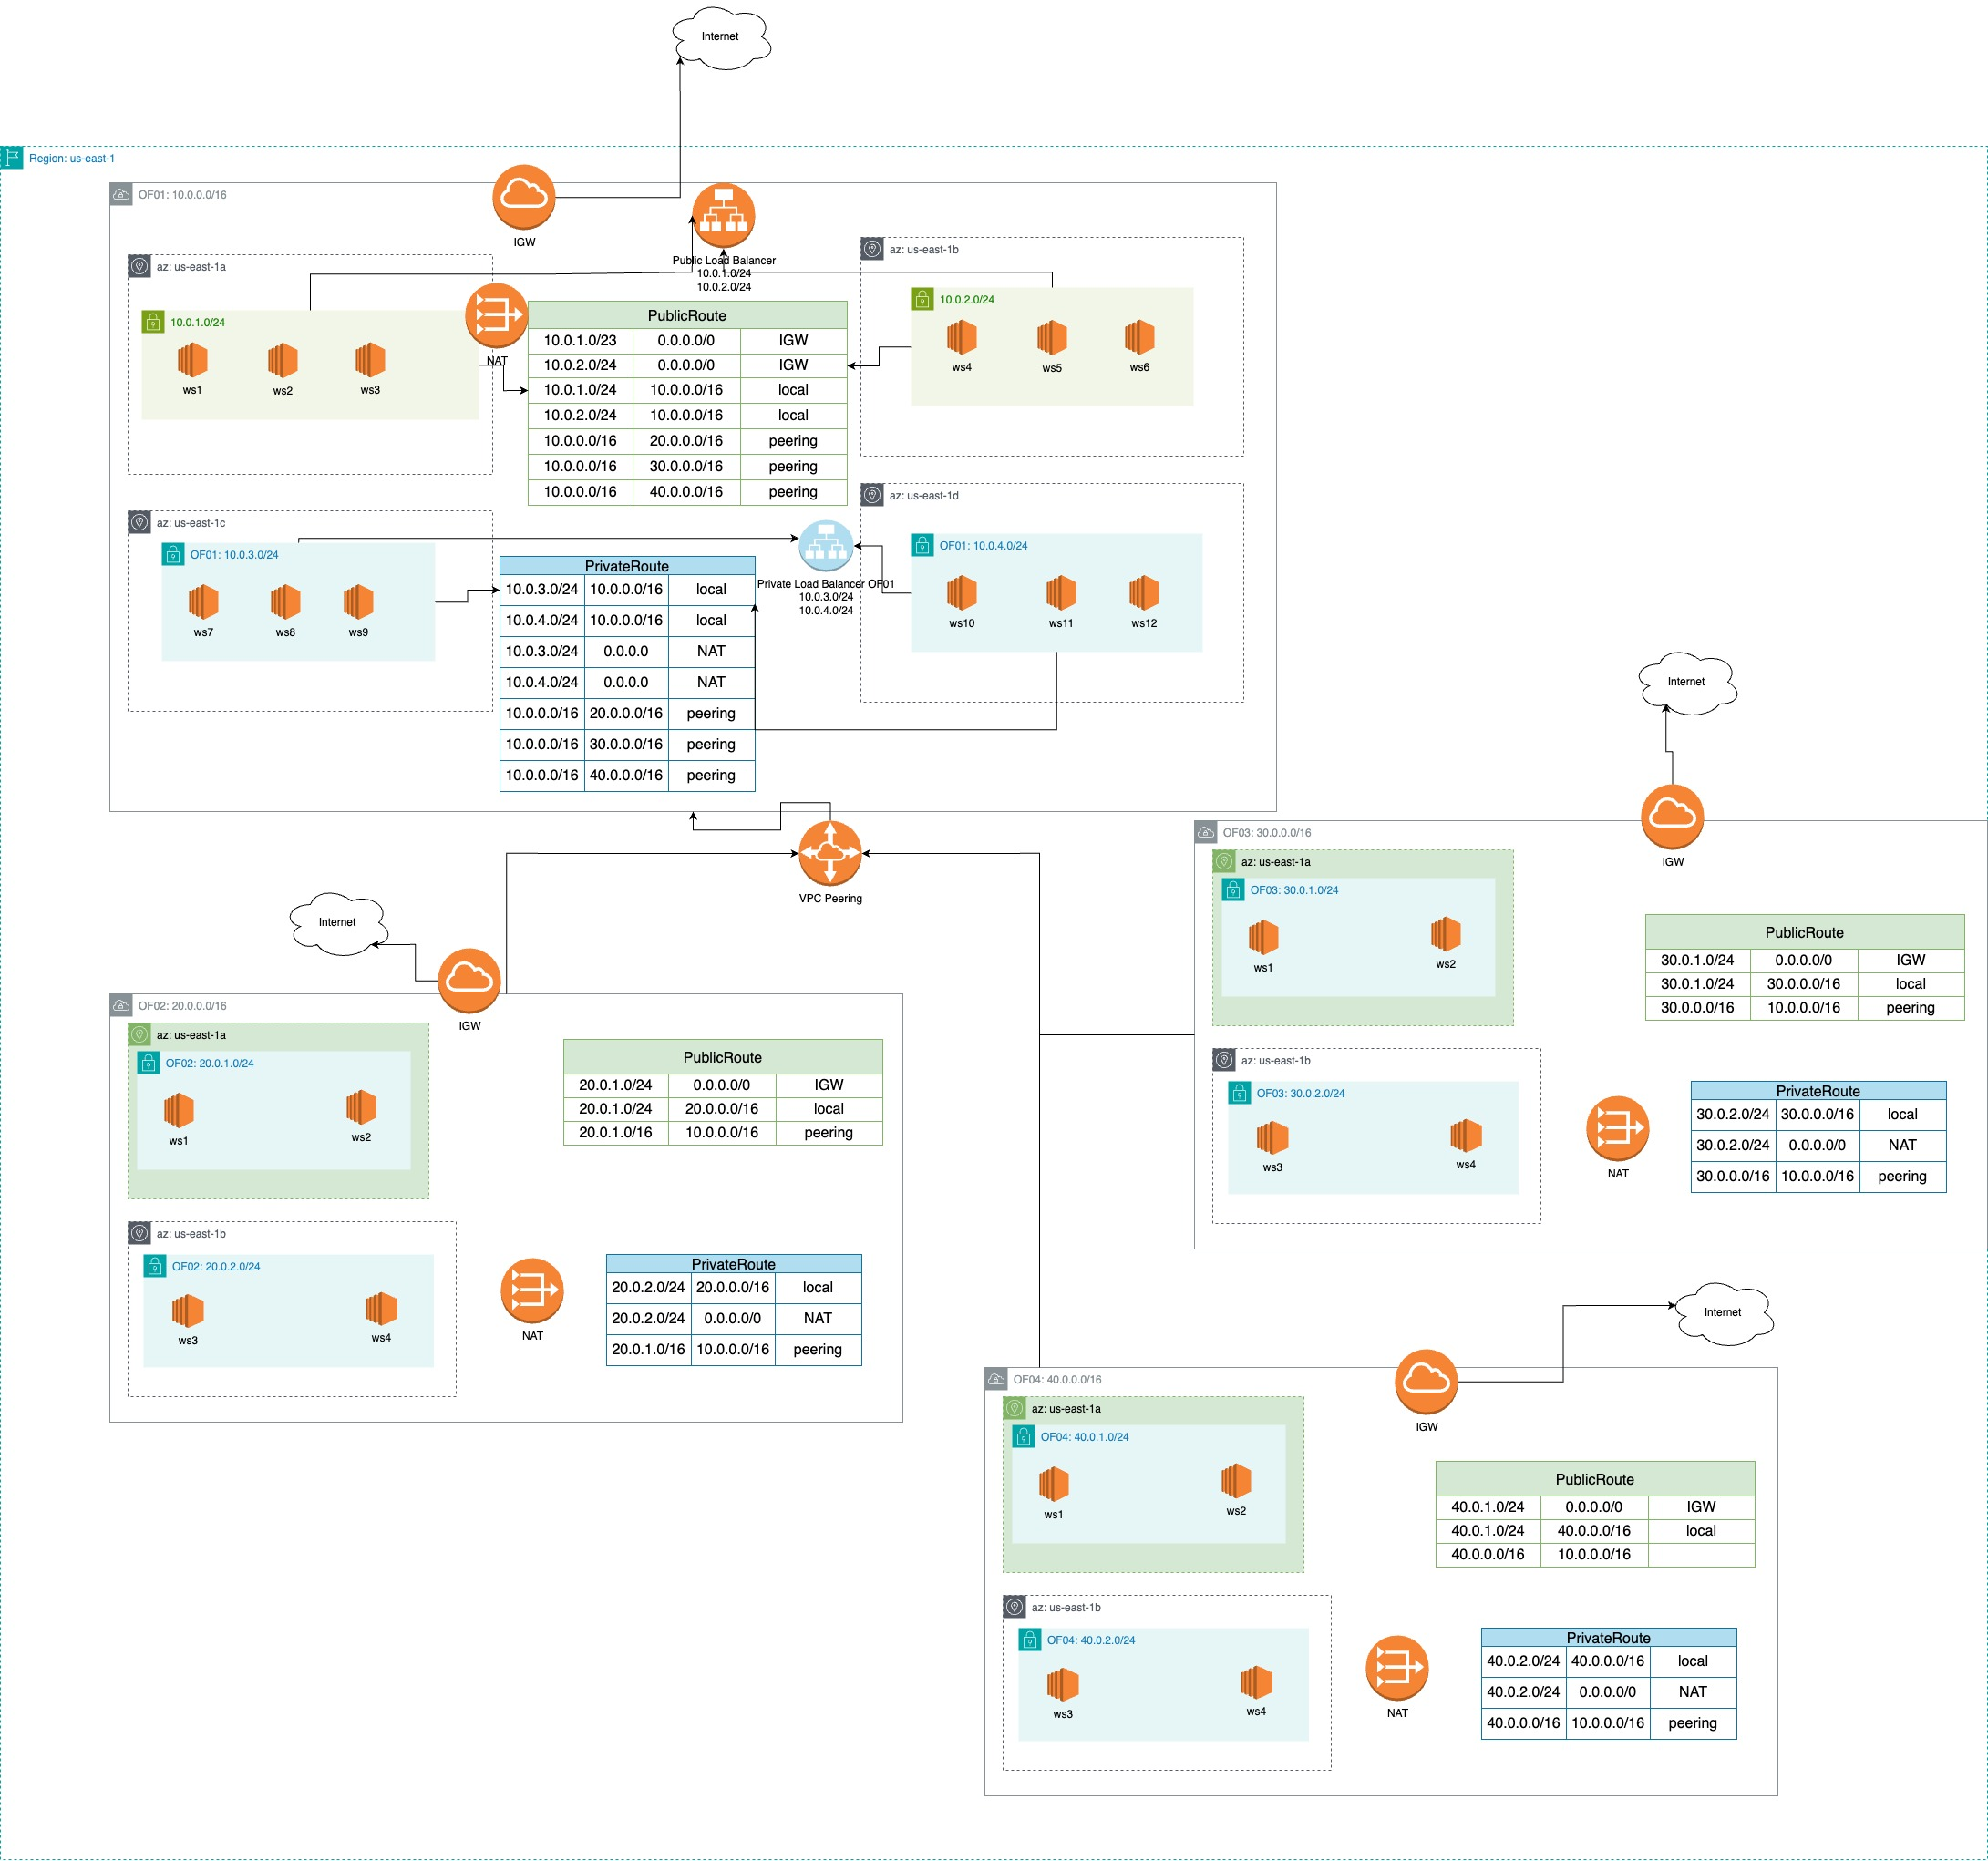
\includegraphics[width=\textwidth]{network_achitecture.jpg}
    \caption{Arquitectura de la solución}
\end{figure}

\subsection{Capturas de la configuración}
Adjuntamos las capturas de la configuración de la solución propuesta,
las siguientes se organizarán de la siguiente manera:

\subsubsection{VPC}
\begin{figure}[!h]
    \centering
    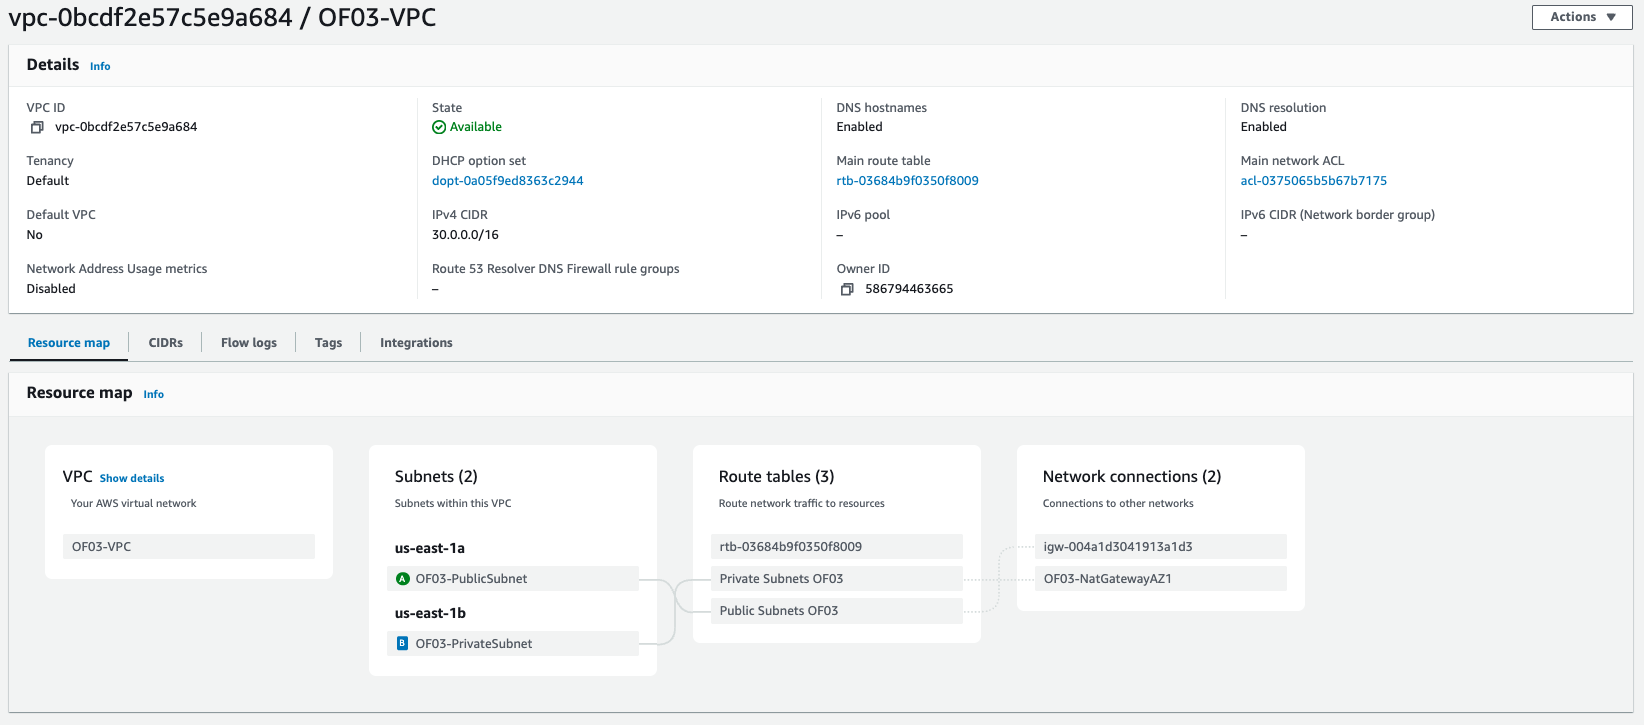
\includegraphics[width=\textwidth]{office1/vpc.png}
    \caption{VPC Oficina Nro 1}
\end{figure}


\subsubsection{Subredes públicas}
\begin{figure}[h!]
    \centering
    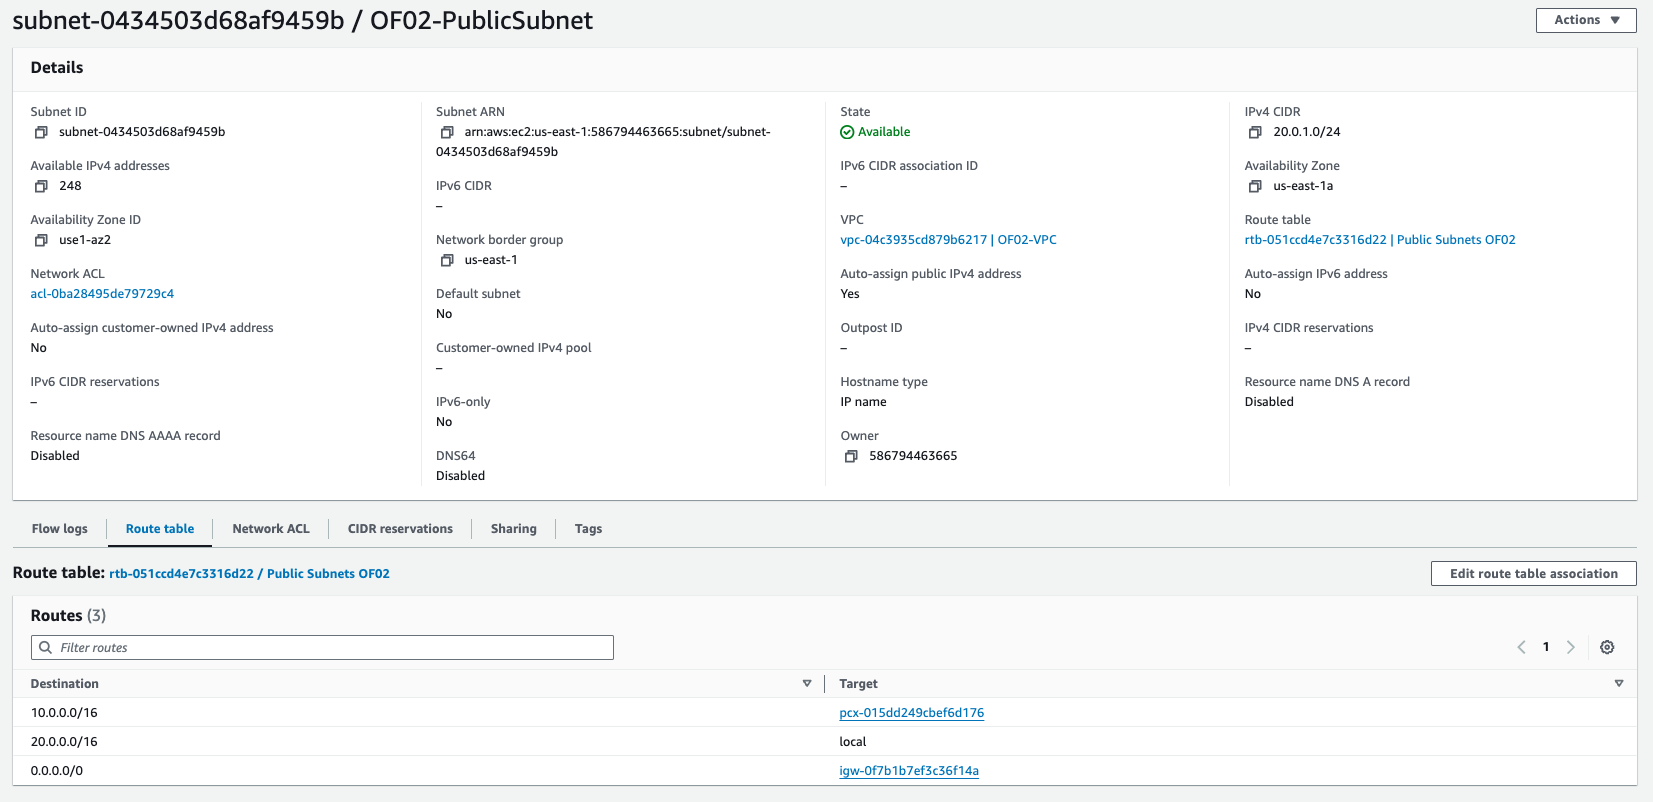
\includegraphics[width=\textwidth]{office1/public_network.png}
    \caption{Subred pública Oficina Nro 1}
\end{figure}


\subsubsection{Subredes privadas}
\begin{figure}[h!]
    \centering
    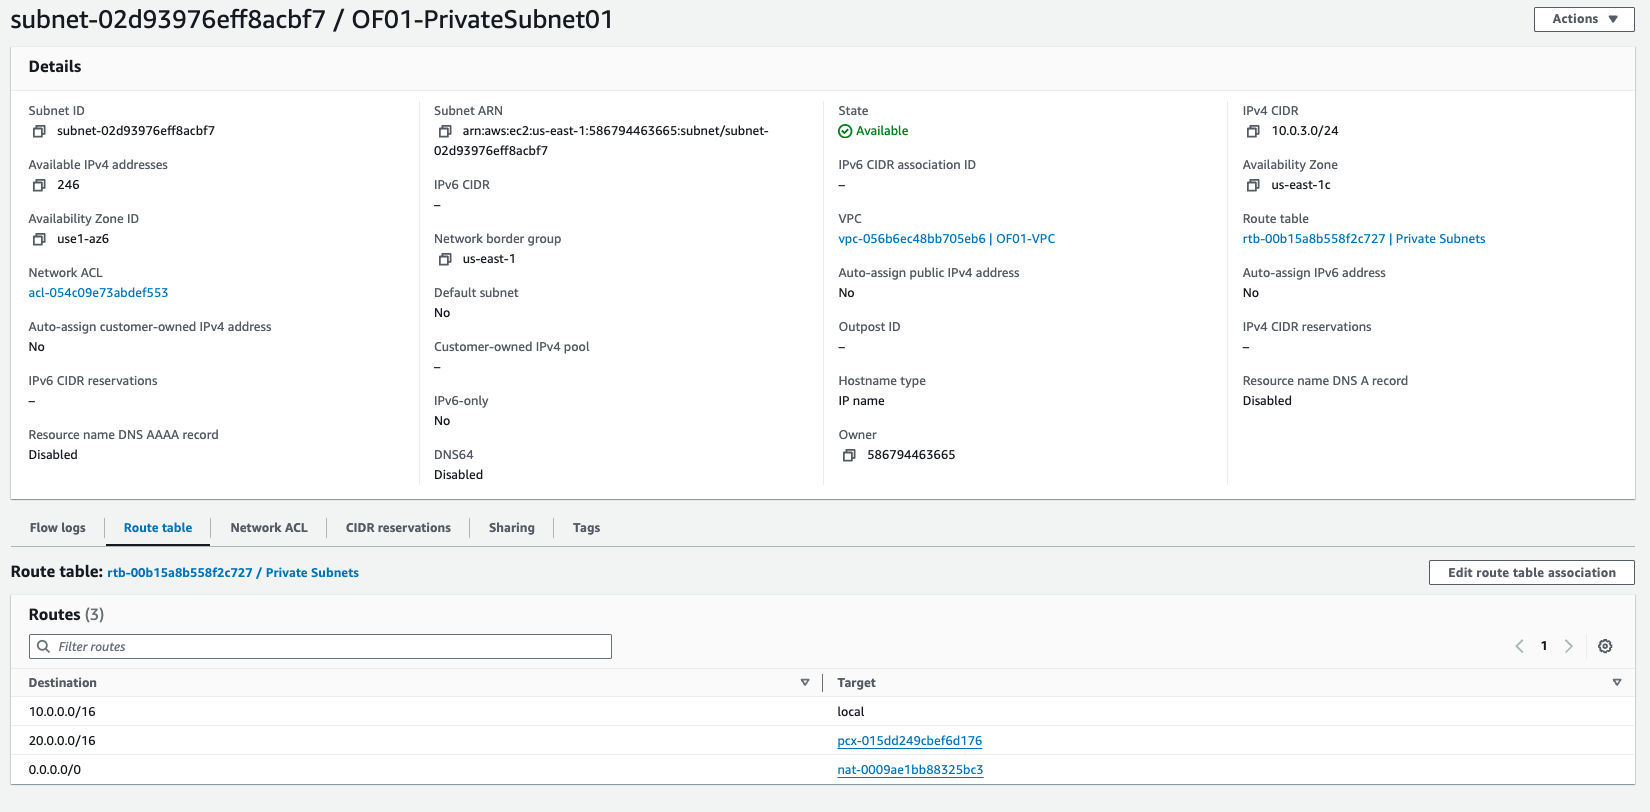
\includegraphics[width=\textwidth]{office1/private_network.png}
    \caption{Subred privada Oficina Nro 1}
\end{figure}


\subsubsection{Load balancer público}
\begin{figure}[h]
    \centering
    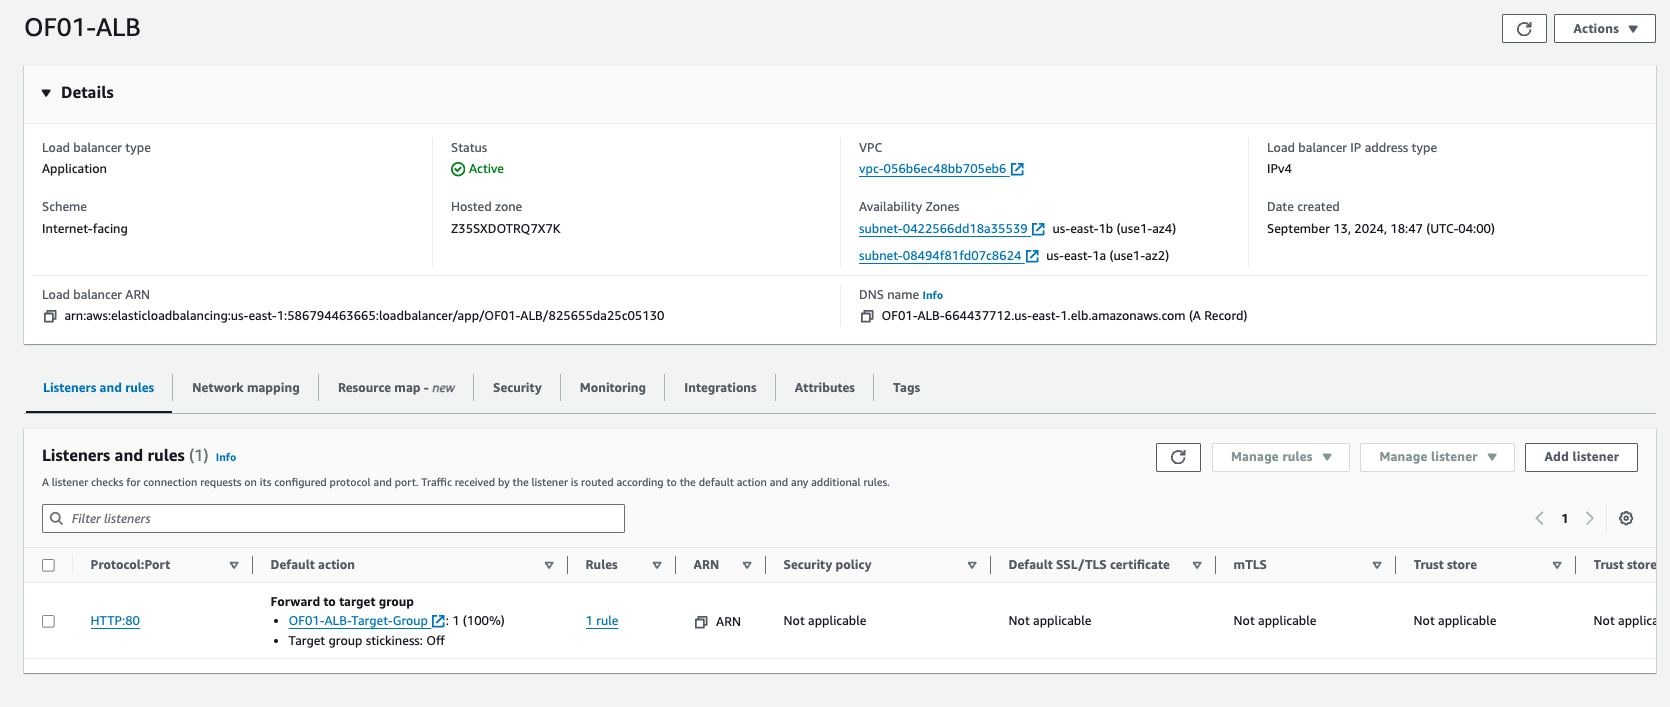
\includegraphics[width=\textwidth]{office1/load_balancer_public.png}
    \caption{Load balancer público Oficina Nro 1}
\end{figure}


\subsubsection{Load balancer privado}
\begin{figure}[h]
    \centering
    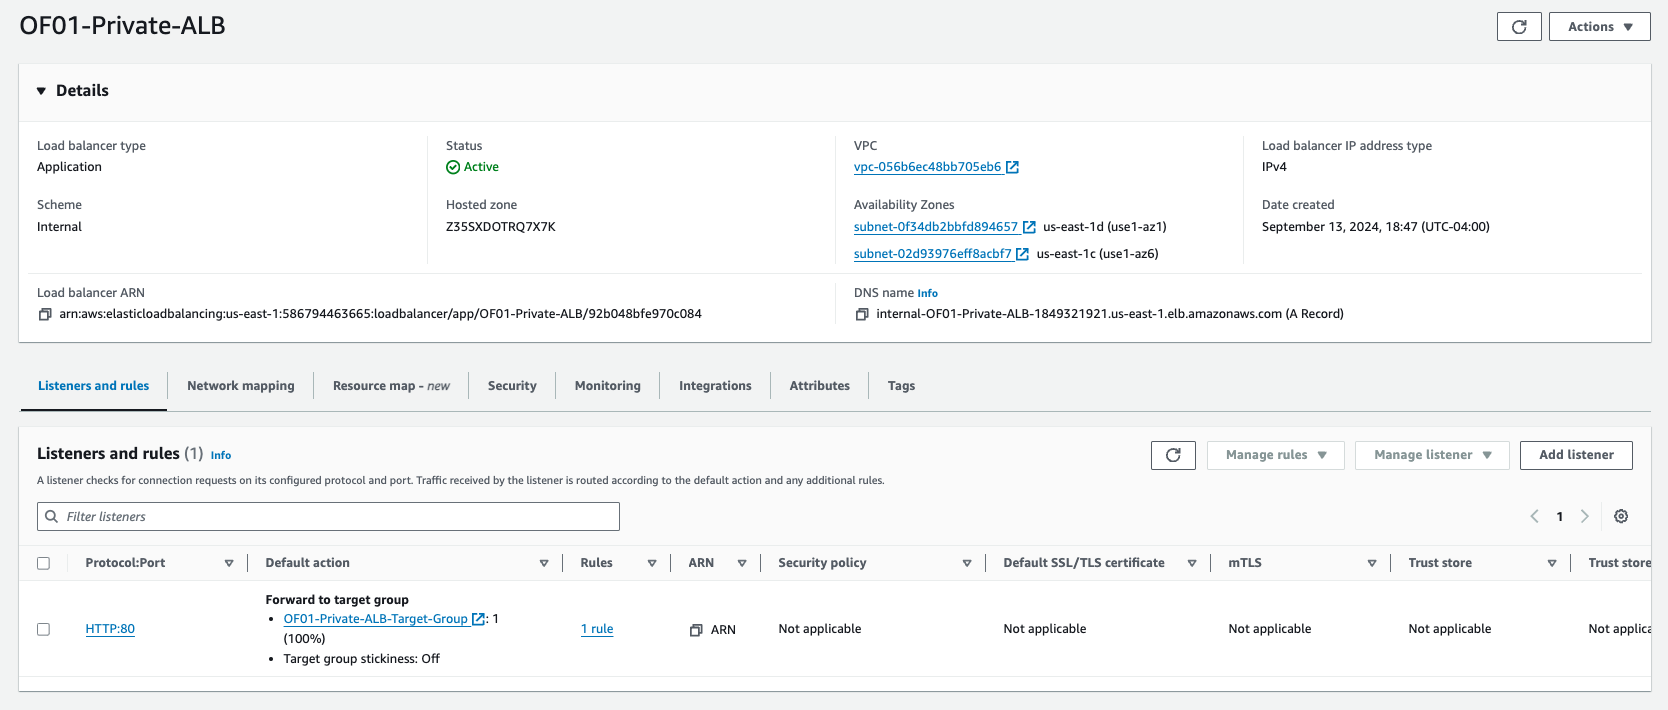
\includegraphics[width=\textwidth]{office1/load_balancer_private.png}
    \caption{Load balancer privado Oficina Nro 1}
\end{figure}


\subsubsection{Internet gateway}
\begin{figure}[h]
    \centering
    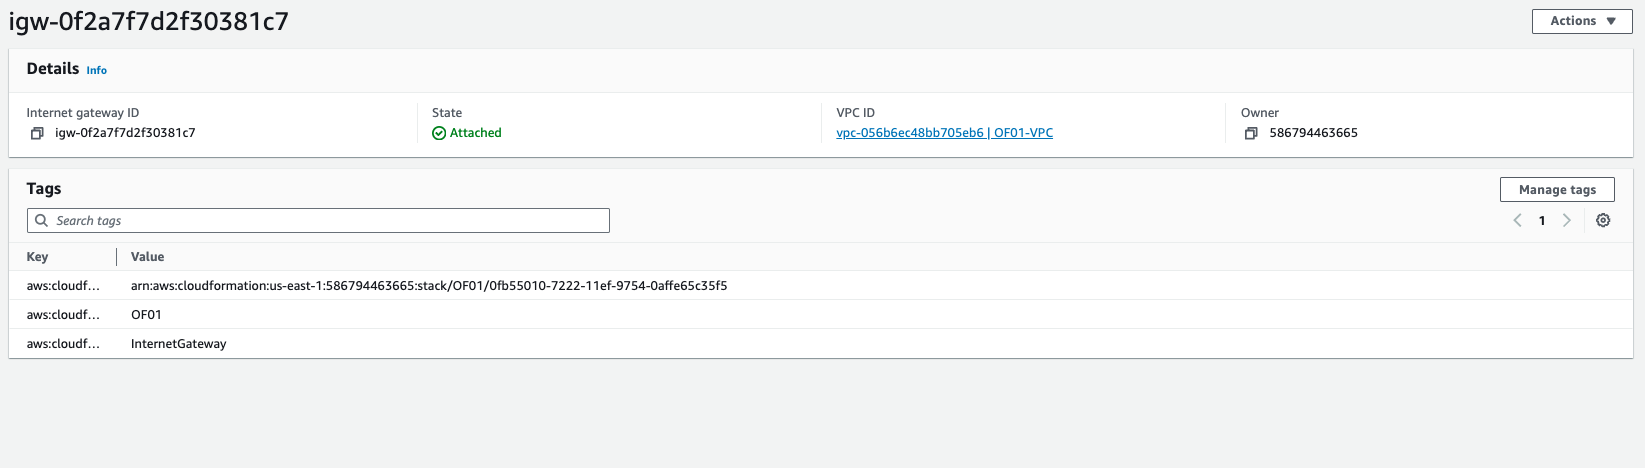
\includegraphics[width=\textwidth]{office1/internet_gateway.png}
    \caption{Internet gateway Oficina Nro 1}
\end{figure}

\subsubsection{Nat gateway}
\begin{figure}[h]
    \centering
    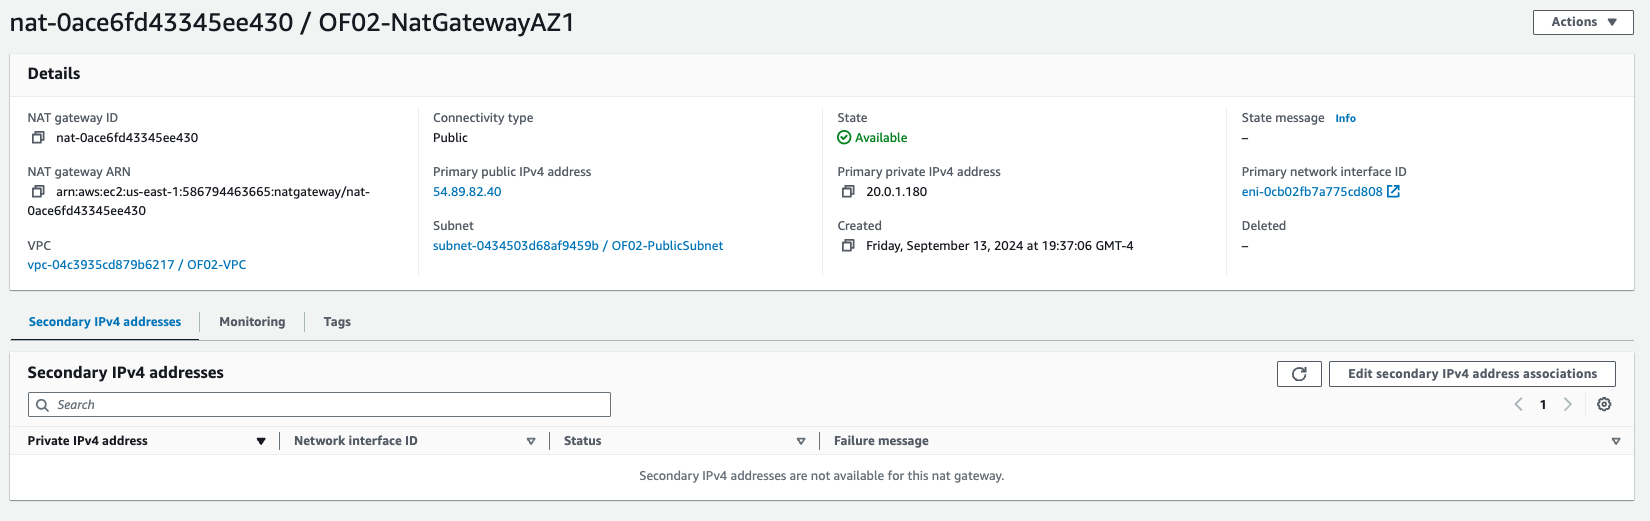
\includegraphics[width=\textwidth]{office1/nat_gateway.png}
    \caption{Nat gateway Oficina Nro 1}
\end{figure}


\subsubsection{EC2}
\begin{figure}[h]
    \centering
    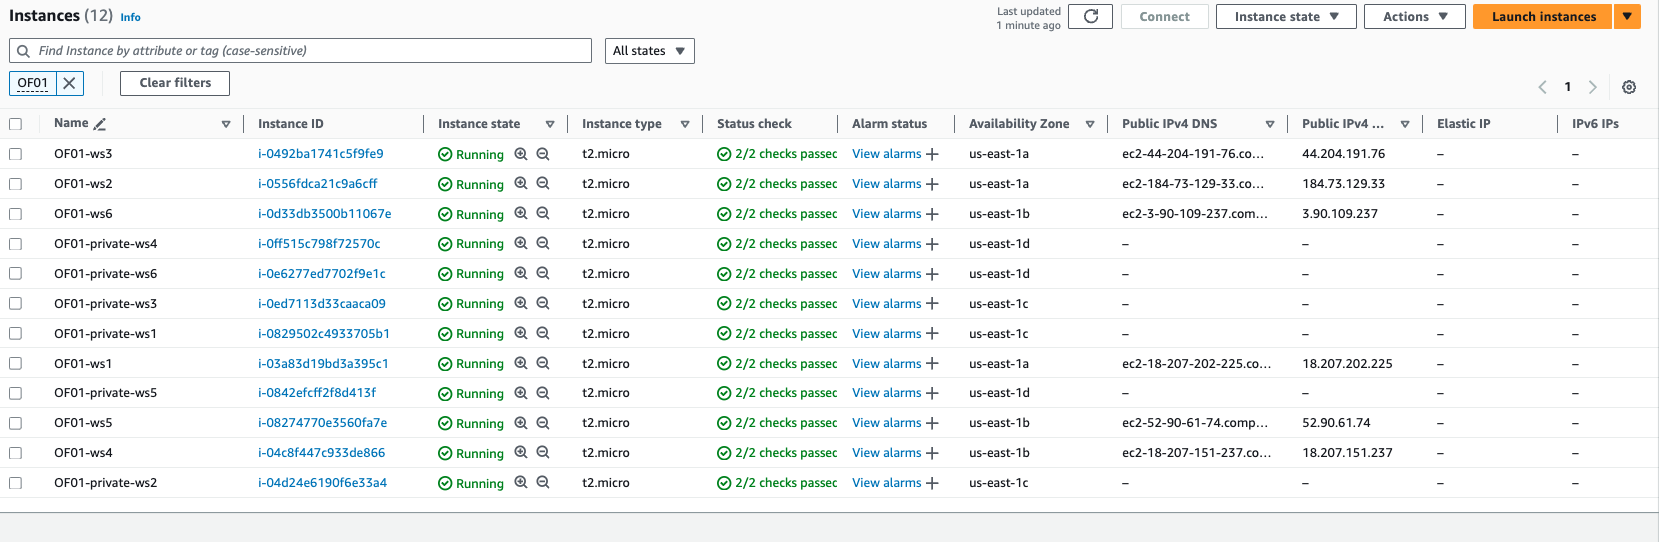
\includegraphics[width=\textwidth]{office1/ec2.png}
    \caption{EC2 Oficina Nro 1}
\end{figure}

\subsubsection{Peering connections}
